%% Template para dissertação/tese na classe UFBAthesis
%% versão 0.9.2
%% (c) 2005 Paulo G. S. Fonseca
%% (c) 2012 Antonio Terceiro
%% www.dcc.ufba.br/~terceiro/ufbathesis

\documentclass[msc, a4paper, classic, en]{ufbathesis}
\usepackage[utf8]{inputenc}
\usepackage[super]{nth}

%% Preâmbulo:
%% coloque aqui o seu preâmbulo LaTeX, i.e., declaração de pacotes,
%% (re)definições de macros, medidas, etc.

\title{A multi-view environment for markerless augmented reality}
\date{December \nth{15}, 2014}
\author{Caio Sacramento de Britto Almeida}
\adviser{Antônio Lopes Apolinário Júnior}
% \coadviser{<NOME DO(DA) CO-ORIENTADOR(A)>}

\begin{document}

% Folha de rosto
% FIXME: Check if 0007 is the right sequential number
\dmccfrontpage{MMCC-Msc-0007}
% Se seu trabalho não for uma tese de doutorado do DMCC, apague a linha
% acima e use \frontpage

%%
%% Parte pré-textual
%%
\frontmatter

% Portada (apresentação)
\dmccpresentationpage
% Se seu trabalho não for uma tese de doutorado do DMCC, apague a linha
% acima e use \presenationpage

% Ficha catalográfica
\authorcitationname{Sacramento de Britto Almeida, Caio} % e.g. Terceiro, Antonio Soares de Azevedo
\advisercitationname{Apolinário Jr., Antônio Lopes} % e.g. Chavez, Christina von Flach Garcia
\catalogtype{Thesis (master)} % e.g. ``Tese (doutorado)''
\catalogtopics{1. Multi-view environment. 2. Augmented reality. 3. Computer graphics} % e.g. ``1. Complexidade Estrutural. 2. Engenharia de Software''
% FIXME: Check the CDD
\catalogcdd{CDD 20.ed. 123.45} % e.g. ``CDD 20.ed. XXX.YY'' (esse número vai lhe ser dado pela biblioteca)
\catalogingsheet

% Termo de aprovação - exemplo
% Modifique com os membros da sua banca
\approvalsheet{Salvador, December \nth{15}, 2014}{
  \comittemember{Prof. Dr. Antônio Lopes Apolinário Júnior 1}{Federal University of Bahia - Brazil}
  \comittemember{Prof. Dr. Michelle Ângelo 2}{State University of Feira de Santana - Brazil}
  \comittemember{Prof. Dr. Rodrigo Silva 3}{Federal University of Juiz de Fora - Brazil}
}

% Agradecimentos
% Se preferir, crie um arquivo à parte e o inclua via \include{}
\acknowledgements
I would like to thank my family for all the support during all those years,
not only the time spent on the master program, but also during all my graduation.
Namely, first I would like to thank my brother, Rodrigo, for being my inspiration on following this career;
my twin sister, Thalita, for being my support of all times;
my parents, for the great education that was given to me;
my grandmother Lourdes; my girlfriend Jéssica; my friends; and specially my advisor Antônio Apolinário
for relying on me to make this work happen.

% Resumo em Português
% Se preferir, crie um arquivo à parte e o inclua via \include{}
%\resumo
% Palavras-chave do resumo em Português
%\begin{keywords}
%\end{keywords}

% Resumo em Inglês
% Se preferir, crie um arquivo à parte e o inclua via \include{}
\abstract
Augmented reality is a technology which allows 2D and 3D computer graphics to be aligned or registered with scenes of the real-world in real-time. This projection of virtual images requires a reference in the captured real image, which is often achieved by using one or more markers. But, there are situations where using markers can be unsuitable, like medical applications, for example. In this work, we present a multi-view environment, composed by augmented reality glasses and two Kinect devices, which doesn't use fiducial markers in order to run augmented reality applications. All devices are calibrated according to a common reference system, and then the virtual models are transformed accordingly too. In order to achieve that, two approaches were specified and implemented: one based on one Kinect plus optical flow and accelerometer data from augmented reality glasses, and another one based purely on two Kinect devices. The results regarding quality and performance achieved by these two approaches are presented and discussed, as well as a comparison between them.
\begin{keywords}
augmented reality, augmented reality glasses, kinect, transformation, optical flow, markerless
\end{keywords}

% Sumário
% Comente para ocultar
\tableofcontents

% Lista de figuras
% Comente para ocultar
\listoffigures

% Lista de tabelas
% Comente para ocultar
\listoftables

%%
%% Parte textual
%%
\mainmatter

% É aconselhável criar cada capítulo em um arquivo à parte, digamos
% "capitulo1.tex", "capitulo2.tex", ... "capituloN.tex" e depois
% incluí-los com:
% \include{capitulo1}
% \include{capitulo2}
% ...
% \include{capituloN}
%
% Importante: Use \xchapter ao invés de \chapter, conforme exemplo abaixo.

\xchapter{Introduction}{In this chapter I present the motivation, objectives and overview of this work.}
\section{Motivation}

Augmented reality has taken advantage from the progresses on the fields of multimedia and virtual reality, making feasible new forms of
interaction between humans and machines. Differently from virtual reality, that takes the user to a virtual environment, the augmented
reality keeps the user on his physical environment and takes the virtual environment to the user's space, allowing the interaction with
the virtual world, in a more natural manner and without needing training or adaptation \cite{1}. Many times, this interaction means
merging virtual images with images captured from a real environment.

One of the greatest challenges on the field of augmented reality is to determine, in real time, which virtual image to be displayed,
in which position and how it should be represented. In order to obtain an integration illusion between real objects and virtual objects,
the generated object should be aligned with the tridimensional position and orientation of the real objects \cite{2}. This can be achieved
by estimating the camera position.

On many situations, fiducial markers\footnote{A fiducial marker or fiducial is an object placed in the field of view of an imaging system which appears in the image produced, for use as a point of reference or a measure.} are used (often this is due to the real time requirements of the augmented reality applications) \cite{3} and are drawn in a way that they can be easily identified. Those markers need to be placed on the target scene and can achieve great results using just a few computational resources. Figure \ref{fig:fiducial_marker} shows the usage of a fiducial marker and a tridimensional object being projected over it.

\begin{figure}
\label{fig:fiducial_marker}
\centering
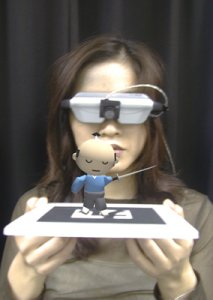
\includegraphics[width=0.3\textwidth]{images/fiducial_marker.png}
\caption{Fiducial marker used to represent a tridimensional model over it \cite{35}}
\end{figure}

However, besides requiring human interference on the scene, there situations where the usage of fiducial markers is not possible, feasible or comfortable for the target model. That is the case, for example, of medical applications on which this model is a patient. It's also possible to cite other limitations of fiducial markers, like, for example, occlusion (a virtual image could be not projected if the marker is not completely visible) and illumination (the intensity of light reflected by the marker could make it hard to be identified). Less common, there are approaches that replace fiducial markers \cite{6} \cite{7} by GPS, gyroscopes, accelerometers, cameras, among others \cite{3} \cite{8}. These approaches have the advantage of not requiring human interference on the scene (to put a marker or to move it around).

Depending on the way that a user sees the mixed world, augmented reality can be classified on two ways. When the user sees the mixed world pointing his eyes straight to the real positions with optical scene or video, this augmented reality is called \textit{immersive} or of \textit{direct vision}. On the other hand, when the user sees the mixed world by some device, like a monitor screen or projector, not aligned with the real positions, this augmented reality is \textit{non-immersive} or of \textit{indirect vision} \cite{1}.

This work proposes a multi-view environment for augmented reality, of direct vision, composed by two Kinects \cite{43} and augmented reality glasses, that allows a watcher visualize, in real time, virtual images merged with real images from the target model. In this approach, it's not intended to use any fiducial marker. Instead, it will be used a geometric approach based on the data captured by each Kinect. This proposed environment can be used, for example, on the medical field (real situations, education and training) or in other situation where a multi-view environment for markerless augmented reality is applicable. 

\section{Objectives}

The environment proposed on this work aims to contribute to augmented reality applications where virtual images need to be merged with real images in real time, without using fiducial markers, and considering the viewing angle of the observer and the position of the target object.

\subsection{Features}

Based on the study of related works, it was defined the following features that define the scope of the first version of the augmented
reality environment, graphically represented on Figure \cite{fig:diagram}:

\begin{figure}
\label{fig:diagram}
\centering
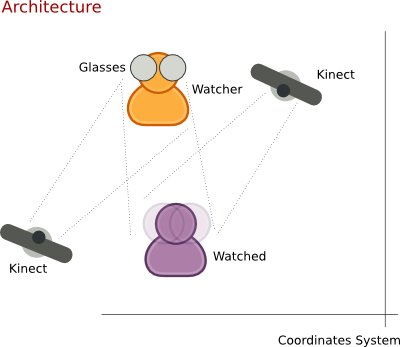
\includegraphics[width=0.3\textwidth]{images/diagram.png}
\caption{Global vision}
\end{figure}

\begin{itemize}
  \item There are two main elements on the environment, the observer and the target model;
  \item Observer and target model are positioned one in front of the other, with some restriction of minimum and maximum distance;
  \item The observer sees the combination of a real image with a pre-defined virtual image over the target model, through the augmented
        reality glasses;
  \item The observer and target model can move their heads, in a way that the virtual image adapts itself in real time to fit the new
        viewing angles;
  \item No fiducial marker is used.
\end{itemize}

The elements presented on this environment are the following:

\begin{itemize}
  \item Observer - He is the user of the system that wears a pair of augmented reality glasses and is positioned in front of the target model (which can be a human being, for example, or a static object). On a medical context, the observer would be a medical specialist, responsible for observing the patient and responsible for analyzing the combination of the real image (part of the patient body) with a virtual image (from magnetic resonance imaging or computed tomography). The observer is able to move his head.
  \item Augmented reality glasses - The augmented reality glasses are wore by the observer and have two cameras. The images captured from the target model will be merged with virtual images and displayed on the two lenses of these glasses. On one of the approches implemented by this work, the observer movimentation is determined from sensors present on the glasses: acceletometer, magnetometer and gyroscopes. Based on sensor data, it's possible to determine the variation on the orientation of the glasses, and so it's possible to know how much the observer has moved his head. This calculation returns values that define moviments on longitudinal axis, vertical axis and lateral axis. The virtual image should be reprojected in real time according to those movements.
  \item Target model - The target model (a human being, for example), is placed in front of the observer and doesn't use any kind of fiducial marker. The main goal is that the virtual image is placed over the target model. In order to calculate where and how the virtual image should be displayed, it's necessary to identify the position and orientation of the real object relative to the observer. This is done based on two sensors placed on the environment, where the first one captures data from the observer and the second one captures data from the target model.
  \item Sensors - Two sensors are placed on the environment and capture data from the observer and the target model (one for each). The information captured by the target model's sensor contains its model, that will be merged with the virtual image.
\end{itemize}

Each device presented on this multi-view (glasses and sensors) environment has its own coordinate system, but all information must be converted to a global coordinate system.

Since there are two sensors and one pair of augmented reality glasses, another objective is to implement two different approaches: one that
uses the augmented reality glasses to determine the observer's pose (based on data from accelerometer and magnetometer) and another one that uses a second Kinect device to determine the observer's pose based on a reconstruction of his model.

\section{Thesis overview}

The next chapter "Conceptual primer" describes some basic theory needed. It also describes the hardwares that are used by this work and how to calibrate them. After that, the "Related work" chapter presents some works related to this one, divided by subject. The third chapter, "Solution architecture", after the theory and related works were presented, explains the steps performed in order to implement the objectives of this work. The results of this implementation are presented on the chapter later, "Results", and finally the conclusions about those results are presented on the last chapter, "Conclusions", where possible future works are also listed.

\xchapter{Conceptual primer}{In this chapter I present the main concepts behind this work.}
\section{Augmented reality}
\subsection{Fiducial markers}
\subsection{Markerless}
\subsection{Direct or indirect vision}
\section{Cameras}
\subsection{Calibration}
\subsection{Parameters}
\subsection{Multi-view}
\section{Sensor-based registration approach}
\subsection{Kinect}
\subsection{Registration}
\subsection{Transformation}
\section{Vision-based registration approach}
\subsection{Optical flow}
\subsection{Lucas-Kanade algorithm}

\xchapter{Related work}{In this chapter I present some related works.}
Cover all the related works, with multiple Kinects, optical flow, markerless augmented reality, medical applications, multi-view environment, reconstruction, etc.
\section{Markerless augmented reality}
\section{Multiple Kinects}
\section{Multi-view environment}

\xchapter{Solution architecture}{In this chapter I explain in details the steps performed in order to implement the objective of this work.}
\section{Environment}
Technologies, machines, SOs, etc.
\section{Calibration}
\subsection{Augmented reality glasses calibration}
\subsection{Initial calibration between Kinects}
\subsection{Initial calibration between Kinect and glasses}
\section{Communication}
Network, sockets, etc.
\section{Transformations}
\section{Method 1: Glasses accelerometer and one Kinect}
Cover Lucas-Kanade algorithm, etc.
\section{Method 2: Two Kinects}
Talk about performance of two Kinfus fighting for a single GPU.
\section{Hybrid approach}
When optical flow has just a few feature points, we switch to the second Kinect.

\xchapter{Result}{In this chaper I present the results of the procedure explained in the previous chapter.}
\section{Scope}
Talk about error propagation.
\section{Analysis}
Talk about performance and alignment results.
\section{Comparison}
Compare methods 1 and 2 with regards to performance and quality.

\xchapter{Conclusions}{In this chapter I discuss the conclusions of this work and list some possibilities of future works.}
\section{Future work}

\backmatter

% Apêndices
% Comente se não houver apêndices
\appendix

% É aconselhável criar cada apêndice em um arquivo à parte, digamos
% "apendice1.tex", "apendice.tex", ... "apendiceM.tex" e depois
% incluí-los com:
% \include{apendice1}
% \include{apendice2}
% ...
% \include{apendiceM}


% Bibliografia
% É aconselhável utilizar o BibTeX a partir de um arquivo, digamos "biblio.bib".
% Para ajuda na criação do arquivo .bib e utilização do BibTeX, recorra ao
% BibTeXpress em www.cin.ufpe.br/~paguso/bibtexpress
\bibliographystyle{abnt-alf}
\bibliography{biblio}

%% Fim do documento
\end{document}
